\documentclass[11pt,a4paper]{article}

\usepackage[margin=1in]{geometry}
\usepackage{amsmath,amssymb}
\usepackage{graphicx}
\usepackage{booktabs}
\usepackage{array}
\usepackage{multirow}
\usepackage{float}
\usepackage{xcolor}
\usepackage{hyperref}
\usepackage{caption}
\usepackage{subcaption}
\usepackage{enumitem}

\hypersetup{
    colorlinks=true,
    linkcolor=blue!60!black,
    citecolor=blue!60!black,
    urlcolor=blue!60!black
}

\graphicspath{{figures/}}

\title{\textbf{Common Fault Modeling, Multi-Fault Simulation, and Machine Learning-Based Health Monitoring of a Laboratory DC Motor}}
\author{DC Motor Health Monitoring Project}
\date{\today}

\begin{document}

\maketitle

\begin{abstract}
This report extends our preliminary DC motor health monitoring study by systematically investigating the most common real-world failure modes of brushed DC motors, embedding them into a physics-based electromechanical, thermal, and vibration simulation, and evaluating machine learning models under both single-fault and randomized simultaneous multi-fault operating scenarios. Compared to our earlier 100\,Hz time-domain baseline (binary accuracy 85.83\%, multi-label macro F1-score 0.7694, friction F1-score 0.4946), upgrading the acquisition model to 500\,Hz with 40 combined time-domain, physics-ratio, higher-order statistical, and Fast Fourier Transform (FFT) spectral features dramatically improves fault separability. On a grouped 75/25 train--test split (zero window leakage), an Extra Trees ensemble achieves 99.39\% accuracy (macro F1 = 0.9933) across 7 single-fault classes and 99.33\% binary accuracy / 0.9620 multi-label macro F1-score (91.33\% exact-match accuracy across all 6 fault flags simultaneously) on a 2,400-window randomized multi-fault dataset containing 0, 1, 2, and 3 concurrent faults. Finally, we present a safe and reversible laboratory fault-induction protocol, a two-stage hybrid strategy to address the lack of destructive physical fault data on college lab hardware, and an itemized Bill of Materials (BOM) tailored to a 220\,V laboratory DC motor. All classification metrics reported herein are simulation-based and do not yet represent experimentally validated hardware accuracy.
\end{abstract}

\tableofcontents
\newpage

%======================================================================
\section{Common DC Motor Faults}
%======================================================================

Brushed DC motors are widely deployed in traction, industrial automation, heavy-duty starters, and university electrical machines laboratories due to their high starting torque and straightforward speed control~\cite{yousefnejad2025,chougule2026}. Literature on DC machine diagnostics highlights that failures stem from a combination of electrical erosion, thermal degradation, and mechanical wear~\cite{yousefnejad2025}. Specifically, brush-commutator wear, sparking, and contact erosion degrade electrical conduction and insulation resistance, while mechanical failures such as bearing defects, rotor unbalance, and shaft misalignment generate characteristic vibration signatures.

Based on literature review and industrial reliability studies, seven common DC motor failure modes were identified for this study. Note that \textbf{Bad Bearings} and \textbf{Motor Bearing Failure} represent progressive early and severe stages of the same mechanical degradation mechanism and are therefore consolidated into a unified \emph{Bearing Fault} class during modeling.

\begin{table}[H]
\centering
\caption{Common brushed DC motor failure modes, physical causes, and primary observable signatures.}
\label{tab:common_faults}
\renewcommand{\arraystretch}{1.2}
\begin{tabular}{@{}p{0.23\textwidth}p{0.35\textwidth}p{0.36\textwidth}@{}}
\toprule
\textbf{Fault Mode} & \textbf{Physical Root Cause} & \textbf{Primary Observable Signatures} \\
\midrule
1. Overload of Motor Windings & Sustained mechanical load torque exceeding rated capacity. & High armature current $I_a$, speed droop, steep casing/winding temperature slope ($dT/dt > 0$). \\
2. Loose Windings & Mechanical loosening of armature/field coils due to thermal cycling or varnish aging. & Electromagnetic force vibration at $2\times$ rectifier/slot frequencies (100/200\,Hz) scaling with $I_a^2$; minor impedance jitter. \\
3. Dirty Commutators \& Brush Wear & Carbon dust, oxidation, worn brushes, or poor spring tension causing arcing/sparking~\cite{yousefnejad2025}. & Elevated and angle-varying brush contact resistance $R_b(\theta)$, high-frequency $dI_a/dt$ current spikes, localized heating. \\
4 \& 6. Bad Bearings $\rightarrow$ Bearing Failure & Lubrication loss, raceway pitting/spalling, or rolling-element wear (early to severe). & Increased viscous friction $B$, periodic vibration impulse trains at Ball Pass Frequencies (BPFO/BPFI), high kurtosis/crest factor, bearing end-bell heating. \\
5. Degraded Winding Insulation Breakdown & Thermal/electrical aging causing reduced insulation resistance or early inter-turn shorts. & Drop in effective $R_a$, $L_a$, and flux constant $K$, elevated circulating current, rapid localized thermal rise, mild 100\,Hz magnetic asymmetry. \\
7. Excessive Vibration & Rotor mass unbalance, shaft/coupling misalignment, or loose base mounting bolts. & Strong sinusoidal vibration peaks at $1\times$ RPM (unbalance) and $2\times$ RPM (misalignment); mild $1\times$ torque ripple. \\
\bottomrule
\end{tabular}
\end{table}

%======================================================================
\section{Ideal Separately Excited DC Motor Simulation}
%======================================================================

To establish a controlled baseline matching a typical 220\,V college Electrical Machines Lab motor, a coupled electromechanical, thermal, and vibration model of a separately excited DC motor is formulated.

\subsection{Governing Physics Equations}

\paragraph{1. Armature Electrical Dynamics}
\begin{equation}
    V_a(t) = R_a(T)\,I_a(t) + L_a \frac{dI_a(t)}{dt} + E_b(t)
    \label{eq:elec}
\end{equation}
where $V_a$ is the applied armature voltage, $I_a$ is the armature current, $L_a$ is the armature inductance, and $E_b$ is the back electromotive force (EMF). Copper resistance varies with temperature $T$ according to:
\begin{equation}
    R_a(T) = R_{a,0}\left[1 + \alpha_{\text{Cu}}\left(T - 25^\circ\text{C}\right)\right], \qquad \alpha_{\text{Cu}} = 0.00393\,\text{K}^{-1}
\end{equation}

\paragraph{2. Electromechanical Coupling}
For field voltage $V_f$ (with nominal value $V_{f,\text{nom}} = 220\,\text{V}$), the effective motor constant $K = K_{e,\text{nom}}(V_f / V_{f,\text{nom}})$ links electrical and mechanical variables:
\begin{equation}
    E_b(t) = K\omega(t), \qquad T_e(t) = K I_a(t)
    \label{eq:coupling}
\end{equation}

\paragraph{3. Rotor Mechanical Dynamics}
\begin{equation}
    J \frac{d\omega(t)}{dt} = T_e(t) - T_L(t) - B\omega(t), \qquad \frac{d\theta(t)}{dt} = \omega(t)
    \label{eq:mech}
\end{equation}
where $J$ is rotor inertia, $\omega$ is angular velocity ($\text{rad/s}$), $\theta$ is shaft angle, $T_L$ is external load torque, and $B$ is viscous friction.

\paragraph{4. Lumped Thermal Dynamics}
A first-order lumped thermal model tracks motor casing temperature trends over the monitoring window:
\begin{equation}
    C_{\text{th}} \frac{dT(t)}{dt} = P_{\text{loss}}(t) - \frac{T(t) - T_{\text{amb}}}{R_{\text{th}}}, \qquad P_{\text{loss}} = I_a^2 R_a + B\omega^2 + P_{\text{extra}}
    \label{eq:thermal}
\end{equation}

\paragraph{5. Baseline Vibration and Realistic Supply Non-Idealities}
Even a healthy laboratory motor exhibits non-zero ripple and background vibration. The ideal healthy baseline therefore includes:
\begin{itemize}[noitemsep]
    \item \textbf{Rectifier supply ripple:} $1.2\%$ sinusoidal ripple at $100\,\text{Hz}$ (full-wave rectified 50\,Hz mains).
    \item \textbf{Baseline mechanical vibration:} Small normal $1\times$ RPM ($0.03\text{--}0.07\,g$) and $2\times$ RPM ($0.01\text{--}0.03\,g$) components plus broadband Gaussian accelerometer noise ($\sigma \approx 0.04\,g$).
    \item \textbf{Unit-to-unit parameter tolerance:} $\pm 3\text{--}6\%$ random variation in nominal $R_a, L_a, K, B$, plus realistic sensor measurement noise on $V_a, I_a$, RPM, and $T$.
\end{itemize}

\subsection{Nominal Parameters and Sampling Configuration}

Unlike our previous 100\,Hz model, the upgraded simulator samples at \textbf{$f_s = 500\,\text{Hz}$} ($\Delta t = 2\,\text{ms}$) with 4 internal integration sub-steps per sample for numerical stability ($L_a/R_a \approx 20.8\,\text{ms}$). Each 4-second steady-state run is segmented into two 2-second windows ($N = 1000$ samples/window), providing a Nyquist frequency of 250\,Hz—sufficient to resolve $1\times$/$2\times$ RPM harmonics, 100/200\,Hz electromagnetic chatter, and bearing resonance bands.

\begin{table}[H]
\centering
\caption{Nominal 220\,V separately excited DC motor parameters and randomized operating ranges.}
\label{tab:nominal_params}
\begin{tabular}{@{}llll@{}}
\toprule
\textbf{Parameter} & \textbf{Symbol} & \textbf{Nominal / Range} & \textbf{Units} \\
\midrule
Armature Resistance & $R_{a,0}$ & $1.20$ ($\pm 4\%$ tolerance) & $\Omega$ \\
Armature Inductance & $L_a$ & $0.025$ ($\pm 4\%$ tolerance) & H \\
Nominal Motor Constant & $K_{e,\text{nom}}$ & $1.25$ & $\text{V}\cdot\text{s/rad}$ \\
Rotor Moment of Inertia & $J$ & $0.040$ & $\text{kg}\cdot\text{m}^2$ \\
Viscous Friction Coefficient & $B$ & $0.008$ ($\pm 6\%$ tolerance) & $\text{N}\cdot\text{m}\cdot\text{s/rad}$ \\
Thermal Capacitance / Resistance & $C_{\text{th}}, R_{\text{th}}$ & $220.0,\; 0.45$ & $\text{J/K},\; \text{K/W}$ \\
Randomized Armature Voltage & $V_a$ & $180\text{--}220$ & V \\
Randomized Field Voltage & $V_f$ & $190\text{--}220$ & V \\
Randomized Normal Load Torque & $T_L$ & $8\text{--}18$ & $\text{N}\cdot\text{m}$ \\
Ambient Temperature & $T_{\text{amb}}$ & $25\text{--}30$ & $^\circ\text{C}$ \\
Sampling Rate / Window Size & $f_s,\; T_w$ & $500\,\text{Hz},\; 2.0\,\text{s}$ ($1000$ samples) & -- \\
\bottomrule
\end{tabular}
\end{table}

%======================================================================
\section{Incorporation of Common Faults in the Simulation}
%======================================================================

Each fault $m \in \{1,\dots,6\}$ is parameterized by a continuous severity factor $s_m \in [0.25, 1.0]$ (capturing incipient-to-severe degradation). In the \textbf{randomized multi-fault} formulation, any combination of $k \in \{0, 1, 2, 3\}$ faults can be active simultaneously, and their physical perturbations superpose directly inside the ODE and vibration equations:

\begin{enumerate}[leftmargin=*, itemsep=4pt]
    \item \textbf{Winding Overload ($s_{\text{ov}}$):} Scales the external load torque $T_L \leftarrow T_L(1.35 + 0.70\,s_{\text{ov}})$ and elevates copper loss weighting by $(1 + 0.15 + 0.25\,s_{\text{ov}})$, producing sustained high $I_a$, speed droop, and steeper thermal rise.
    
    \item \textbf{Loose Windings ($s_{\text{lw}}$):} Adds stochastic micro-jitter $\delta R_a \sim \mathcal{N}(0, (0.04 + 0.08\,s_{\text{lw}})R_a)$ and injects electromagnetic vibration chatter at $100\,\text{Hz}$ and $200\,\text{Hz}$ whose amplitude scales with $I_a^2$ (reflecting Lorentz force $F \propto I^2$):
    \begin{equation}
        a_{\text{lw}}(t) = A_{\text{lw}}(s_{\text{lw}})\,\text{clip}\!\left(\left(\frac{I_a}{15}\right)^2, 0.3, 2.5\right)\left[0.65\sin(2\pi \cdot 100t + \phi_1) + 0.35\sin(2\pi \cdot 200t + \phi_2)\right]
    \end{equation}
    
    \item \textbf{Dirty Commutator / Brush Wear ($s_{\text{cm}}$):} Adds an angle-dependent brush contact resistance modulated by $N_{\text{bar}} = 16$ commutator segments plus random sparking spikes occurring with probability $p_{\text{spark}} = 0.015 + 0.045\,s_{\text{cm}}$:
    \begin{equation}
        R_b(\theta, t) = R_{b,0}(s_{\text{cm}})\left[1 + 0.35\sin(16\theta)\right] + R_{\text{arc}}(t)
    \end{equation}
    along with mild bar-pass brush chatter vibration.
    
    \item \textbf{Bearing Fault ($s_{\text{brg}}$, covering Bad Bearings $\rightarrow$ Failure):} Increases viscous friction $B \leftarrow B(1.7 + 2.8\,s_{\text{brg}})$, adds localized bearing heat $P_{\text{brg}} = 25 + 75\,s_{\text{brg}}\,\text{W}$, and injects a periodic Gaussian impulse train at the Ball Pass Frequency Outer race ($\text{BPFO} = 3.58\,f_{\text{shaft}}$, typical of a 6205 bearing) exciting a $165\,\text{Hz}$ structural resonance:
    \begin{equation}
        a_{\text{brg}}(t) = A_{\text{brg}}(s_{\text{brg}})\,\exp\!\left(-\frac{(\psi_{\text{bpfo}} - \pi)^2}{2(0.18)^2}\right)\sin(2\pi \cdot 165t), \quad \psi_{\text{bpfo}} = (3.58\,\theta) \bmod 2\pi
    \end{equation}
    
    \item \textbf{Degraded Winding Insulation ($s_{\text{ins}}$, Early Inter-Turn Short Proxy):} Models a shorted winding fraction $f_s = 0.08 + 0.18\,s_{\text{ins}}$, reducing effective parameters $R_a \leftarrow R_a(1 - f_s)$, $L_a \leftarrow L_a(1 - 1.2 f_s)$, and $K \leftarrow K(1 - 0.65 f_s)$, while adding localized circulating-current heating ($+0.45\text{ to }1.35\times I_a^2 R_a$) and a mild $100\,\text{Hz}$ electromagnetic asymmetry hum.
    
    \item \textbf{Excessive Vibration ($s_{\text{vib}}$, Unbalance / Misalignment / Looseness):} Amplifies synchronous $1\times$ RPM unbalance ($+0.35\text{ to }1.20\,g$) and $2\times$ RPM misalignment ($+0.22\text{ to }0.77\,g$) vibration components alongside a small $1\times$ shaft-frequency torque ripple $T_{L,\text{rip}} = (0.4 + 0.9\,s_{\text{vib}})\sin(\theta)$.
\end{enumerate}

%======================================================================
\section{Simulation Results and Feature Engineering}
%======================================================================

Two datasets were generated to evaluate both isolated fault diagnosis and compound multi-fault identification:
\begin{itemize}[noitemsep]
    \item \textbf{Dataset A (Single-Fault 7-Class):} 980 simulation runs (140 runs/class $\times$ 7 classes = 1,960 windows).
    \item \textbf{Dataset B (Randomized Multi-Fault):} 1,200 simulation runs (2,400 windows) distributed across 0 faults (364 runs), 1 fault (405 runs), 2 simultaneous faults (313 runs), and 3 simultaneous faults (118 runs).
\end{itemize}

\subsection{Simulated Time-Domain and Spectral Signatures}

Figure~\ref{fig:single_signals} illustrates how the seven states separate cleanly across current, vibration FFT, and temperature rise. Figure~\ref{fig:multi_signals} demonstrates how simultaneous fault combinations superpose in Dataset B, producing complex overlapping electrical and spectral profiles.

\begin{figure}[H]
    \centering
    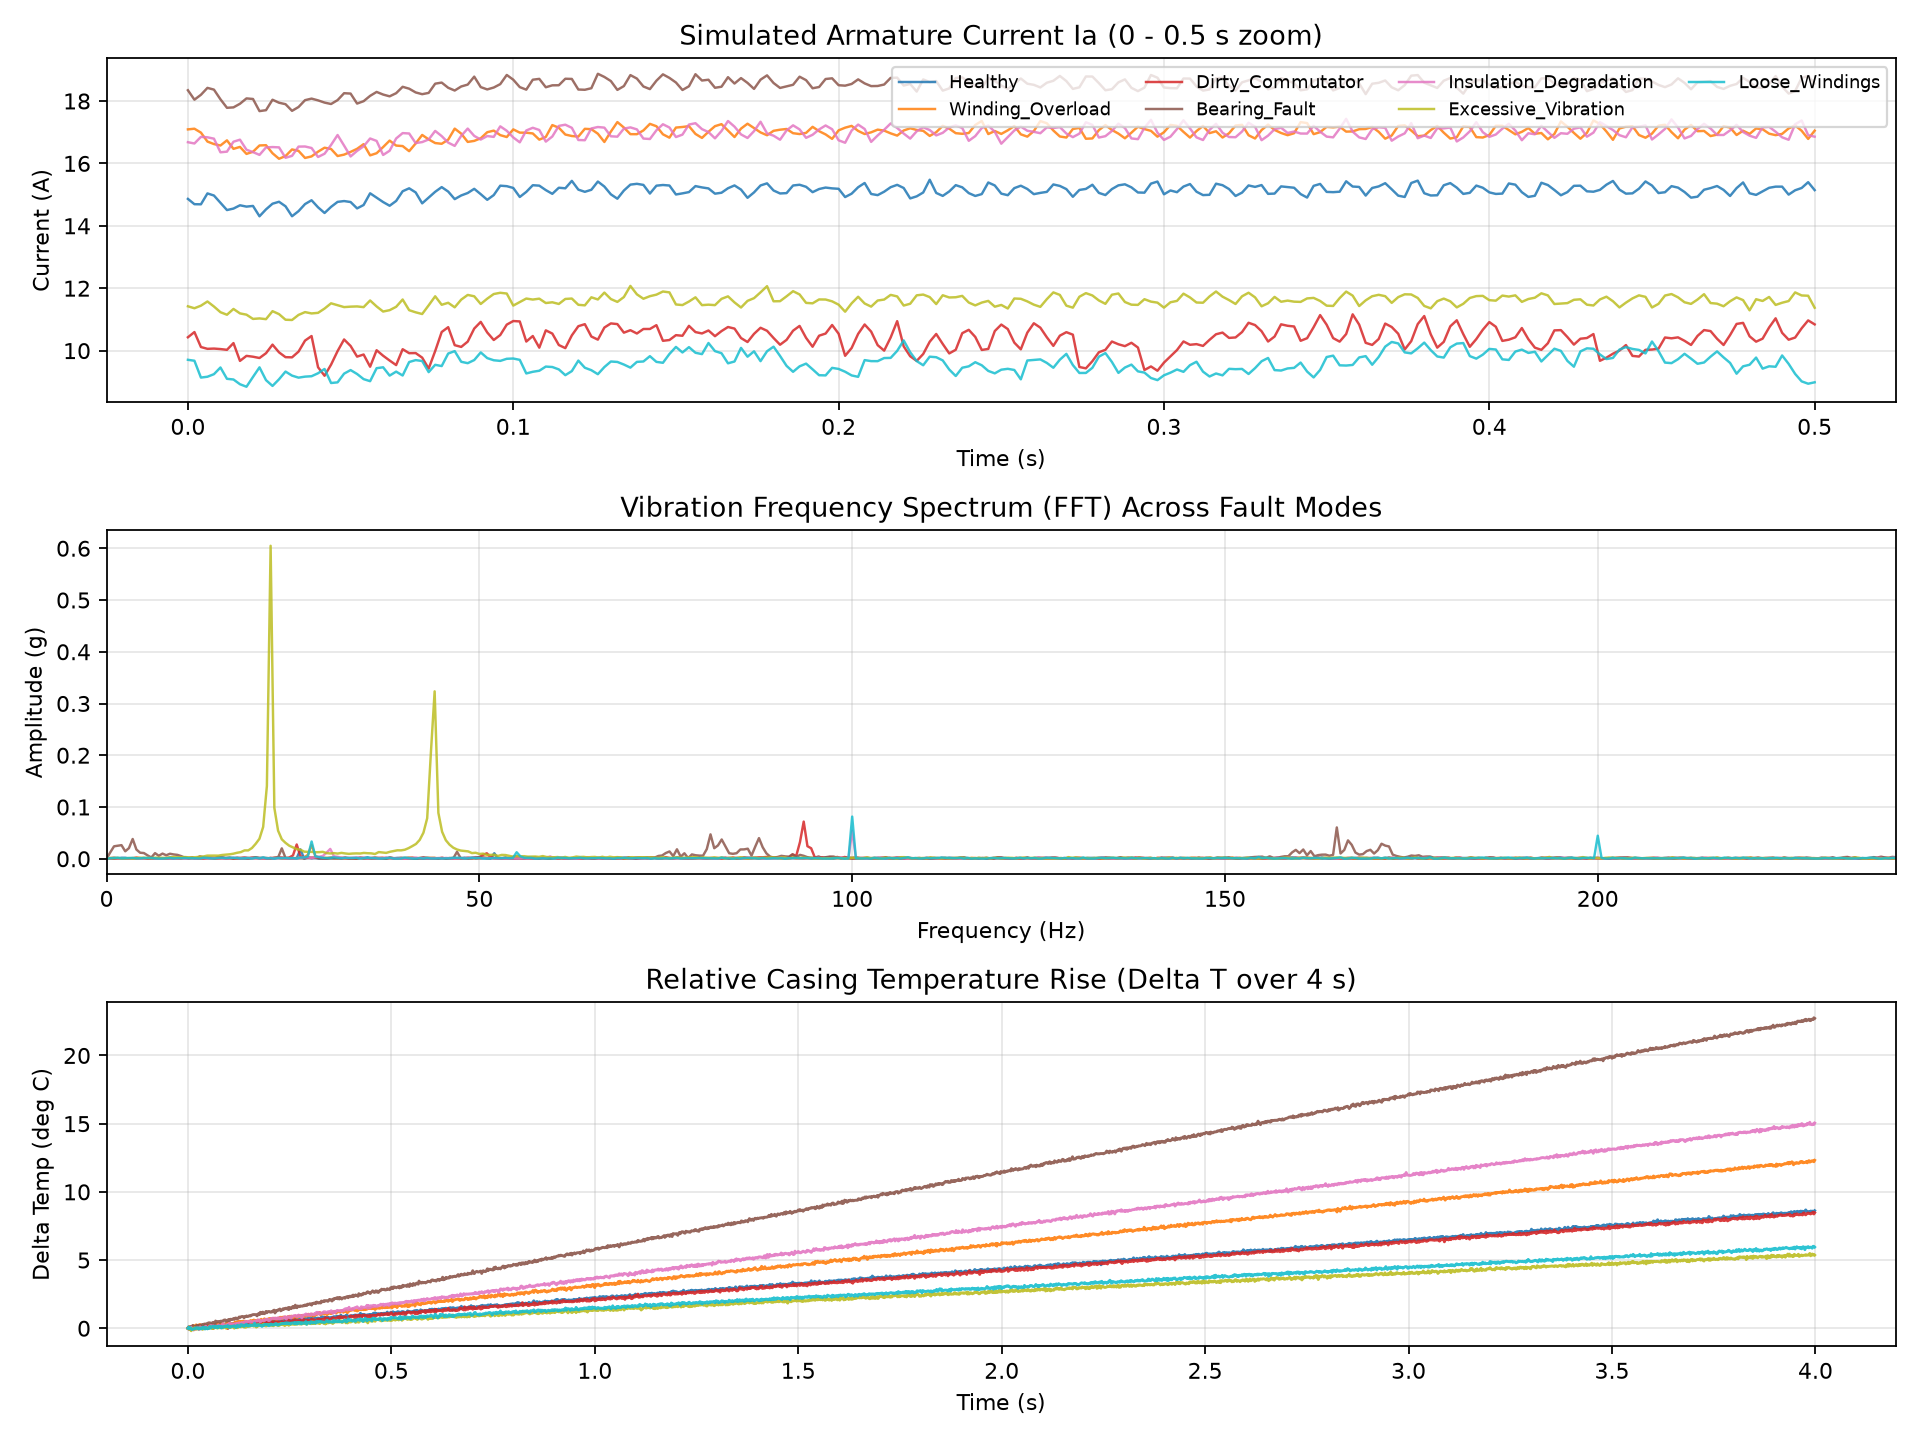
\includegraphics[width=0.95\textwidth]{simulated_signals_comparison.png}
    \caption{Simulated armature current zoom (top), 0--240\,Hz vibration FFT spectrum (middle), and relative casing temperature rise (bottom) across Healthy operation and all six individual fault modes.}
    \label{fig:single_signals}
\end{figure}

\begin{figure}[H]
    \centering
    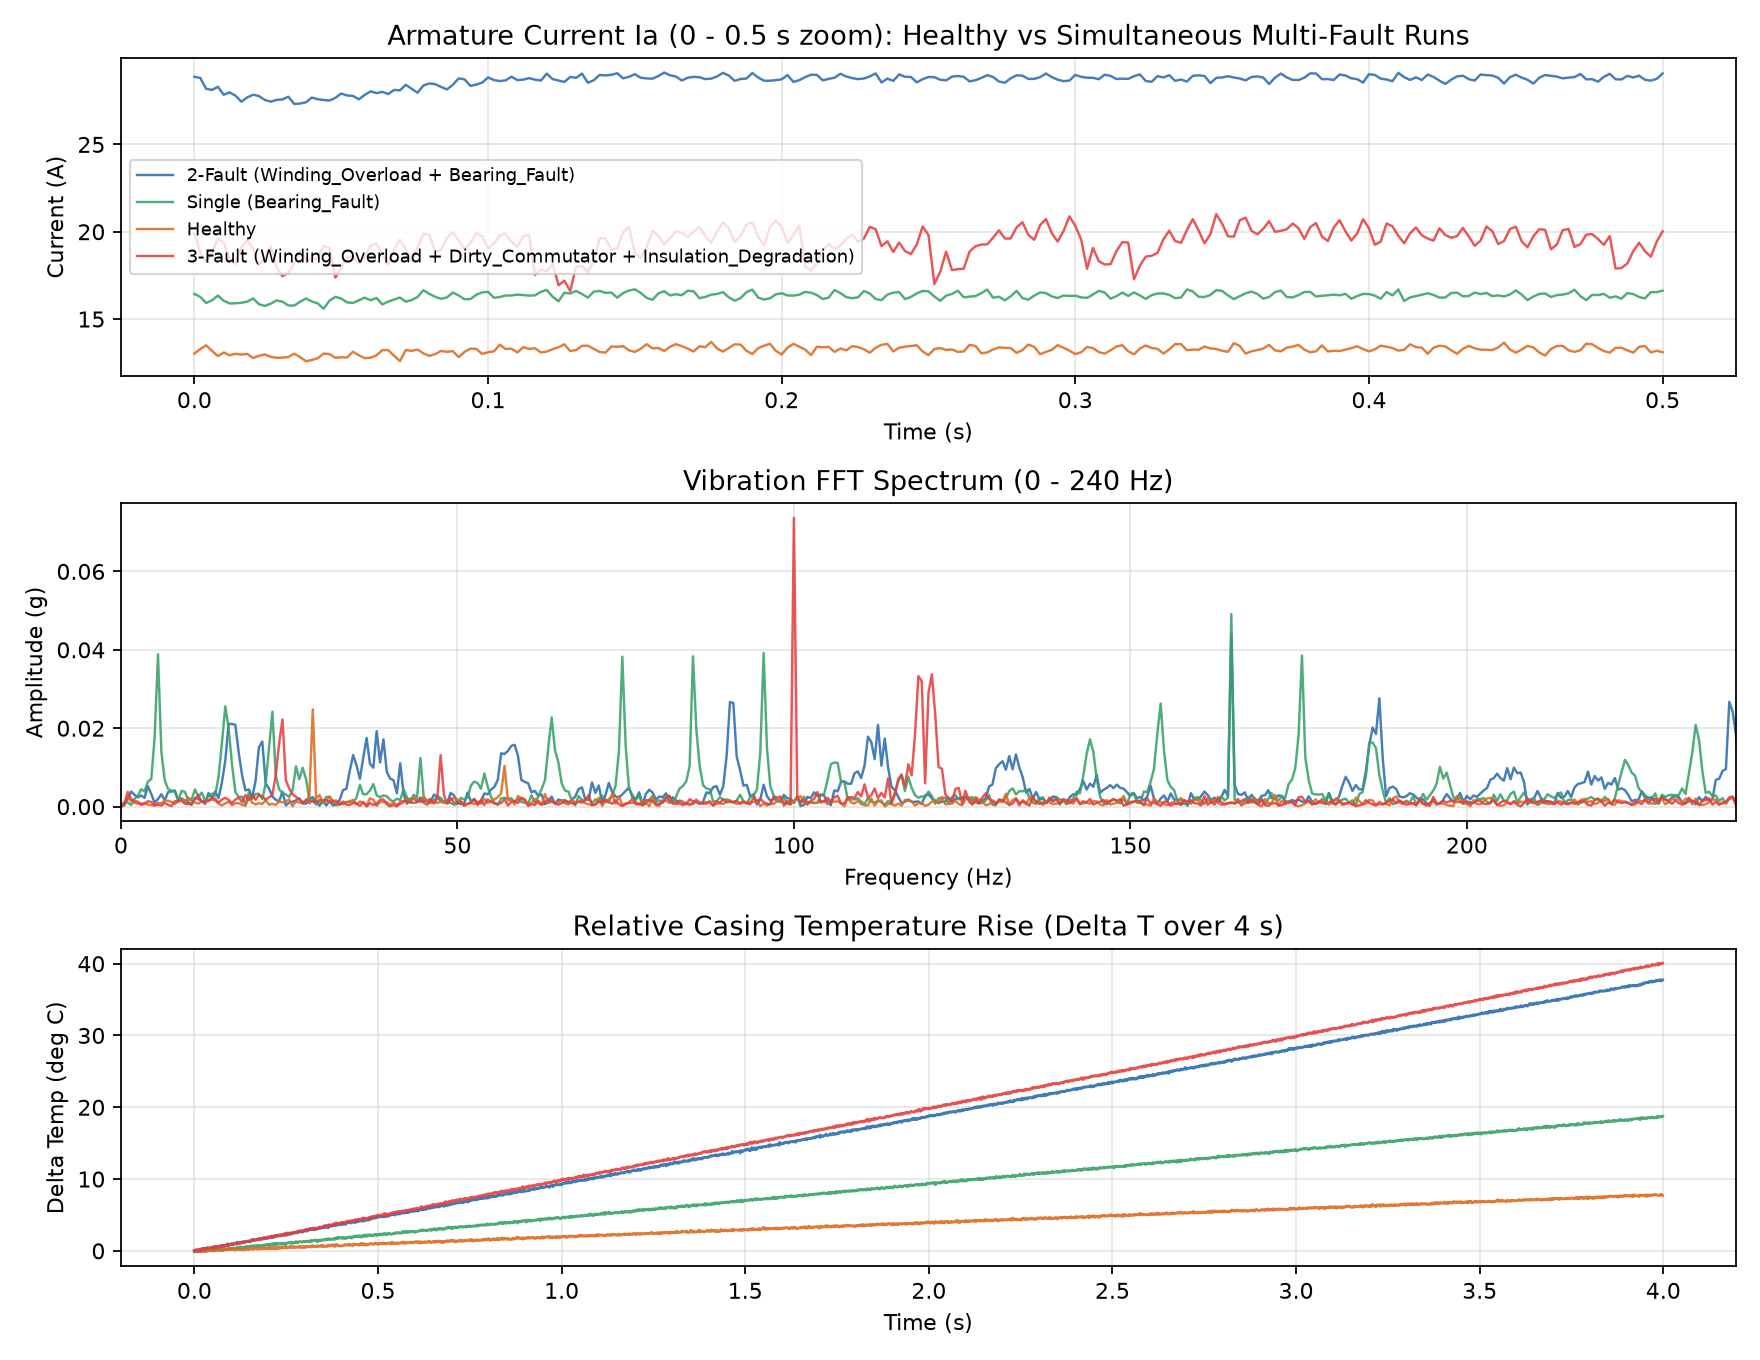
\includegraphics[width=0.95\textwidth]{simulated_multifault_signals.png}
    \caption{Comparison of Healthy operation against randomized 1-fault, 2-fault, and 3-fault simultaneous combinations in the multi-fault dataset.}
    \label{fig:multi_signals}
\end{figure}

\subsection{Feature Extraction (40 Physics + Time + FFT Features)}

From each 2-second window (1,000 samples at 500\,Hz), 40 engineered features are extracted:
\begin{itemize}[noitemsep]
    \item \textbf{Time-domain statistics (20 features):} Mean, standard deviation, RMS, and peak-to-peak for $V_a$, $I_a$, RPM, Temperature, and Vibration.
    \item \textbf{Thermal \& physics-informed ratios (6 features):} Linear temperature slope ($dT/dt$), input power $\overline{V_a I_a}$, $V_a/\text{RPM}$, $I_a/V_a$, first-difference current RMS ($\sqrt{\overline{\Delta I_a^2}}$, sensitive to commutator sparking), and current kurtosis.
    \item \textbf{Higher-order vibration statistics (3 features):} Kurtosis, skewness, and crest factor (highly sensitive to periodic bearing impulses).
    \item \textbf{Frequency-domain FFT features (11 features):} Vibration spectral band energies at $1\times$ RPM, $2\times$ RPM, $100\,\text{Hz}$, $200\,\text{Hz}$, bearing resonance band ($130\text{--}190\,\text{Hz}$), total spectral energy, three normalized band-energy ratios, plus armature current FFT energy at $100\,\text{Hz}$ and high frequency ($120\text{--}240\,\text{Hz}$).
\end{itemize}

%======================================================================
\section{Machine Learning Models and Results}
%======================================================================

\subsection{Model Selection and Validation Protocol}

We selected \textbf{Extra Trees (Extremely Randomized Trees)} ensembles for both binary health detection and multi-label fault identification (`MultiOutputClassifier`) for three reasons:
\begin{enumerate}[noitemsep]
    \item \textbf{High performance on tabular physical features:} Tree ensembles handle nonlinear feature interactions and mixed physical units without scaling, resist overfitting via randomized split thresholds, and execute inference in milliseconds.
    \item \textbf{Interpretability:} Built-in feature importances directly verify that the classifier relies on physically meaningful signatures (vibration kurtosis, FFT bands, $dI_a/dt$, and $dT/dt$).
    \item \textbf{Direct continuity:} Keeping the same classifier family as our previous 100\,Hz report isolates the performance gain achieved by upgrading the physical modeling, 500\,Hz sampling, and FFT feature set.
\end{enumerate}

To prevent data leakage, all evaluations use a \textbf{grouped 75/25 train--test split by \texttt{run\_id}}, ensuring that both 2-second windows from any simulation run reside strictly in either training or testing.

\subsection{Single-Fault 7-Class Classification Results (Dataset A)}

Evaluated on 490 held-out test windows, the 7-class Extra Trees classifier (300 trees) achieved \textbf{99.39\% accuracy}, \textbf{99.30\% balanced accuracy}, and \textbf{0.9933 macro F1-score}. Figure~\ref{fig:cm_single} shows near-diagonal separation across all classes, while Figure~\ref{fig:feat_imp} confirms that FFT spectral bands, vibration kurtosis, and current/thermal features drive classification.

\begin{figure}[H]
    \centering
    \begin{subfigure}[b]{0.49\textwidth}
        \centering
        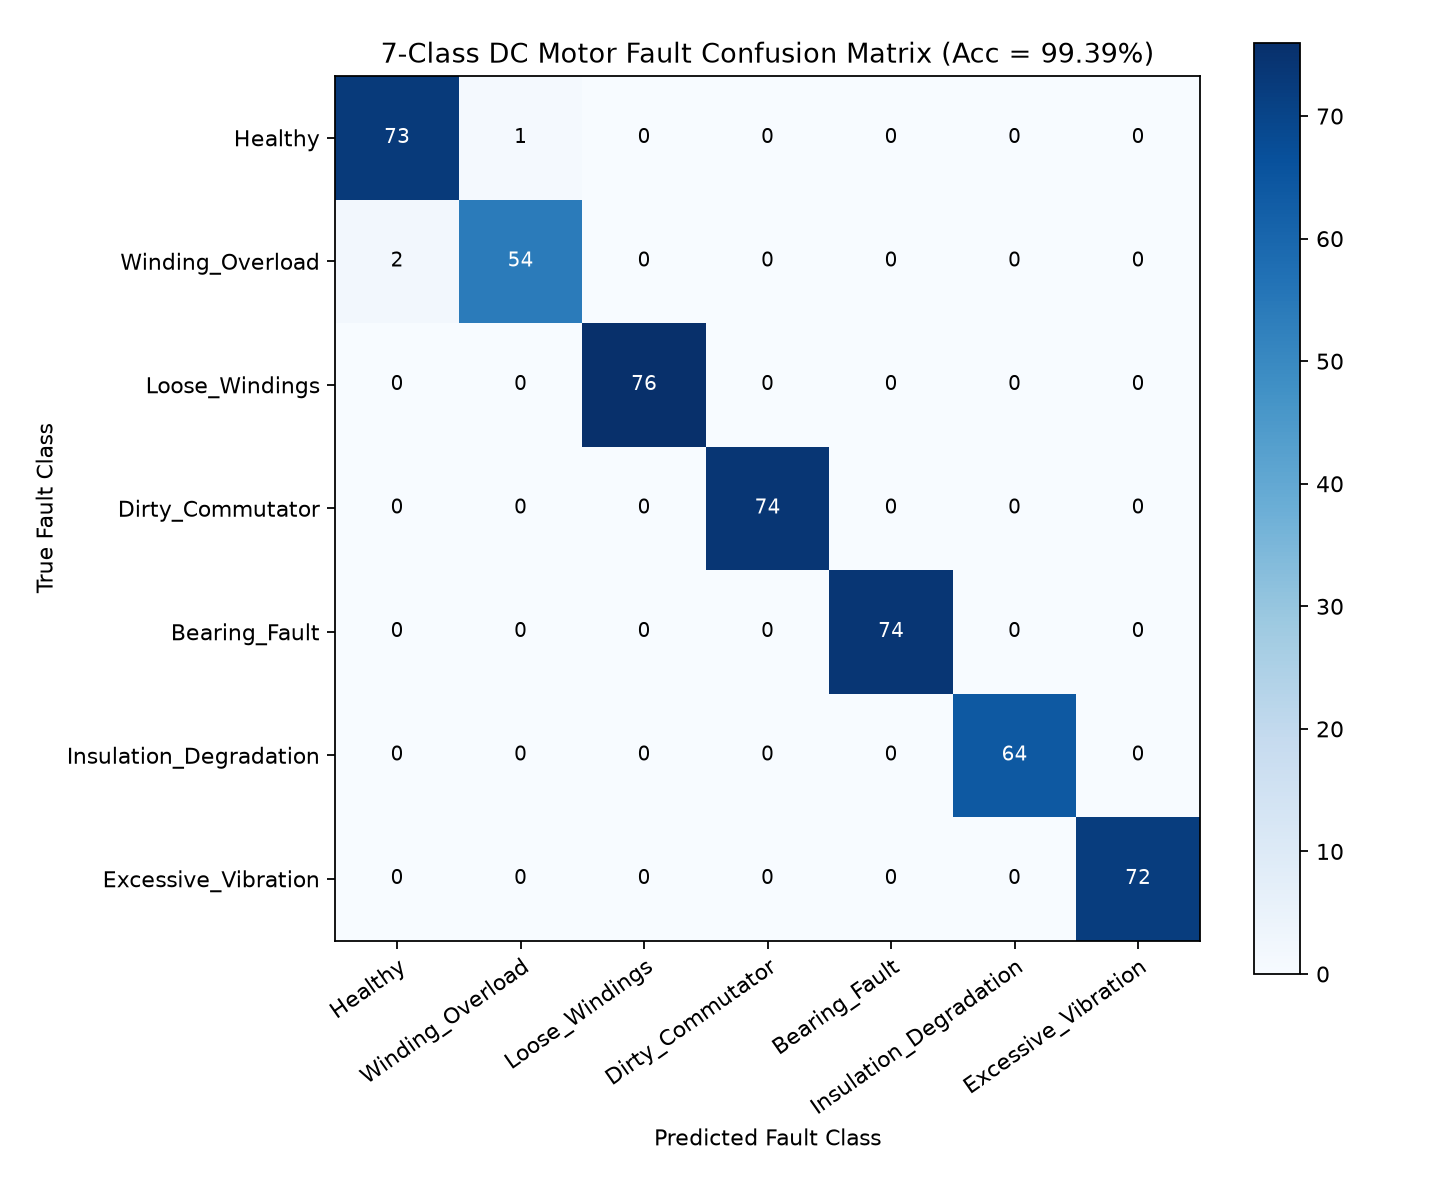
\includegraphics[width=\textwidth]{confusion_matrix_multiclass.png}
        \caption{7-class confusion matrix (Acc = 99.39\%).}
        \label{fig:cm_single}
    \end{subfigure}
    \hfill
    \begin{subfigure}[b]{0.49\textwidth}
        \centering
        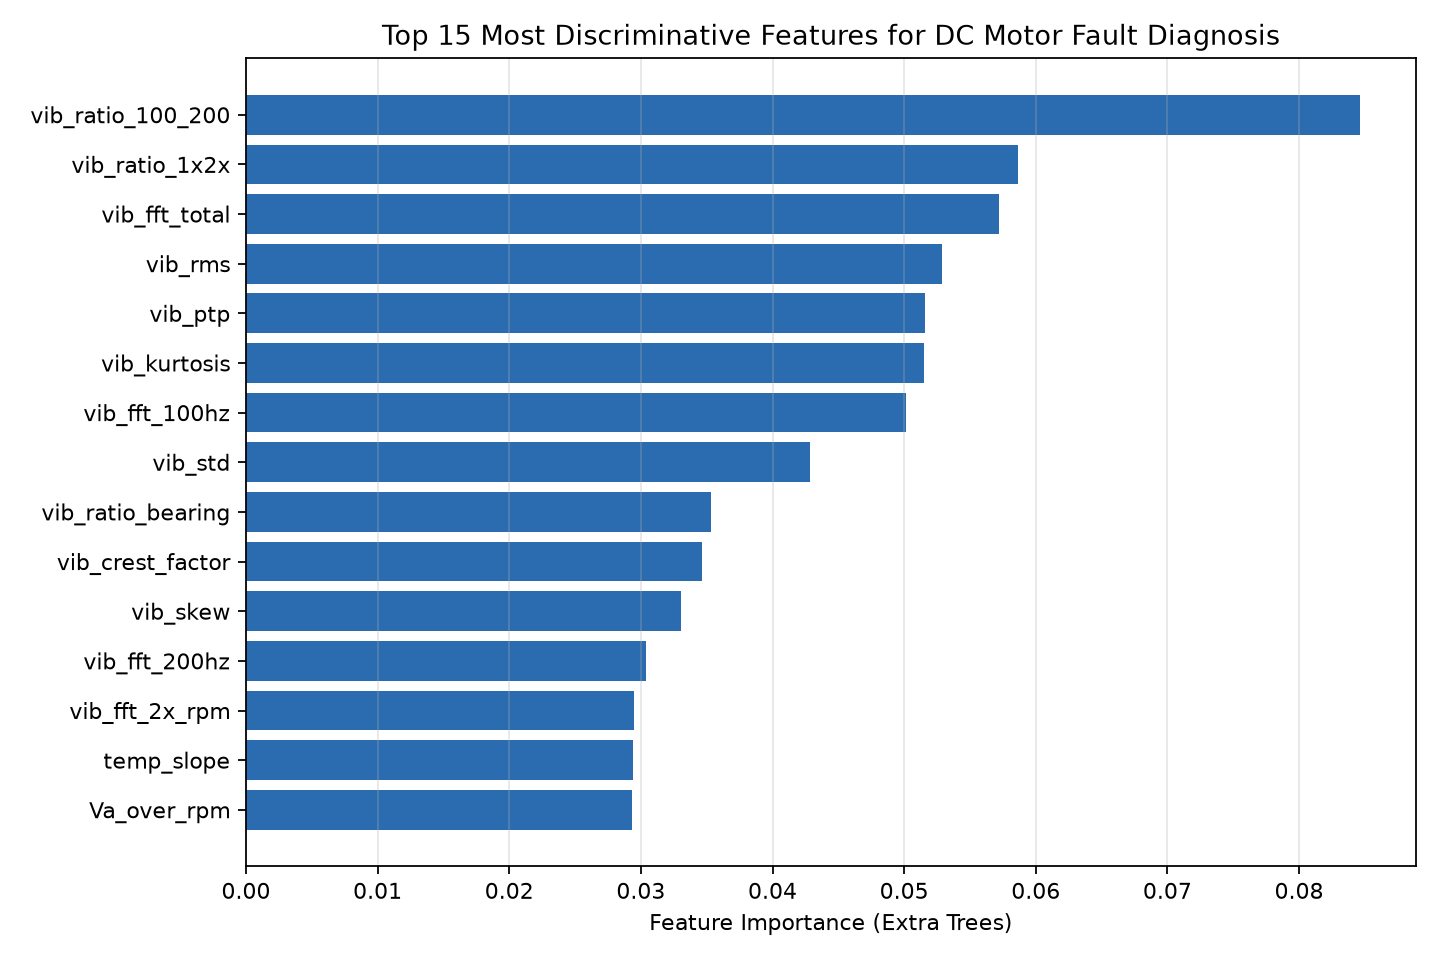
\includegraphics[width=\textwidth]{feature_importance.png}
        \caption{Top 15 Extra Trees feature importances.}
        \label{fig:feat_imp}
    \end{subfigure}
    \caption{Single-fault classification performance and physical feature importance ranking.}
\end{figure}

\subsection{Randomized Multi-Fault Classification Results (Dataset B)}

Evaluated on 600 held-out test windows (containing 0, 1, 2, and 3 concurrent faults):
\begin{itemize}[noitemsep]
    \item \textbf{Binary Health Classifier (250 trees):} Accuracy = \textbf{99.33\%}, Balanced Accuracy = \textbf{99.53\%}, Macro F1 = \textbf{0.9920} (Healthy Recall: 100.00\%, Abnormal Recall: 99.06\%).
    \item \textbf{Multi-Label Fault Identifier (200 trees/output):} Macro F1 = \textbf{0.9620}, Exact-Match Accuracy (all 6 flags simultaneously correct) = \textbf{91.33\%}, Hamming Accuracy = \textbf{98.53\%}.
\end{itemize}

\begin{table}[H]
\centering
\small
\setlength{\tabcolsep}{5pt}
\caption{Per-fault multi-label identification performance on 600 held-out multi-fault test windows.}
\label{tab:multilabel_results}
\begin{tabular}{@{}lccccc@{}}
\toprule
\textbf{Fault Type} & \textbf{Precision} & \textbf{Recall} & \textbf{F1-Score} & \textbf{Accuracy} & \textbf{Support} \\
\midrule
Winding Overload & 0.9811 & 0.8000 & 0.8814 & 95.33\% & 130 \\
Loose Windings & 1.0000 & 0.9516 & 0.9752 & 99.00\% & 124 \\
Dirty Commutator & 1.0000 & 0.8729 & 0.9321 & 97.50\% & 118 \\
Bearing Fault & 1.0000 & 1.0000 & 1.0000 & 100.00\% & 114 \\
Insulation Degradation & 1.0000 & 0.9672 & 0.9833 & 99.33\% & 122 \\
Excessive Vibration & 1.0000 & 1.0000 & 1.0000 & 100.00\% & 122 \\
\midrule
\textbf{Macro Average / Overall} & \textbf{0.9969} & \textbf{0.9320} & \textbf{0.9620} & \textbf{98.53\% (Hamming)} & \textbf{600} \\
\bottomrule
\end{tabular}
\end{table}

\begin{table}[H]
\centering
\caption{Exact-match accuracy breakdown by number of simultaneous faults in the test set.}
\label{tab:exact_by_k}
\begin{tabular}{@{}lcc@{}}
\toprule
\textbf{Simultaneous Fault Count} & \textbf{Test Windows} & \textbf{Exact-Match Accuracy} \\
\midrule
0 faults (Healthy) & 174 & 100.00\% \\
1 simultaneous fault & 200 & 94.00\% \\
2 simultaneous faults & 148 & 85.14\% \\
3 simultaneous faults & 78 & 76.92\% \\
\bottomrule
\end{tabular}
\end{table}

\begin{figure}[H]
    \centering
    \begin{subfigure}[b]{0.42\textwidth}
        \centering
        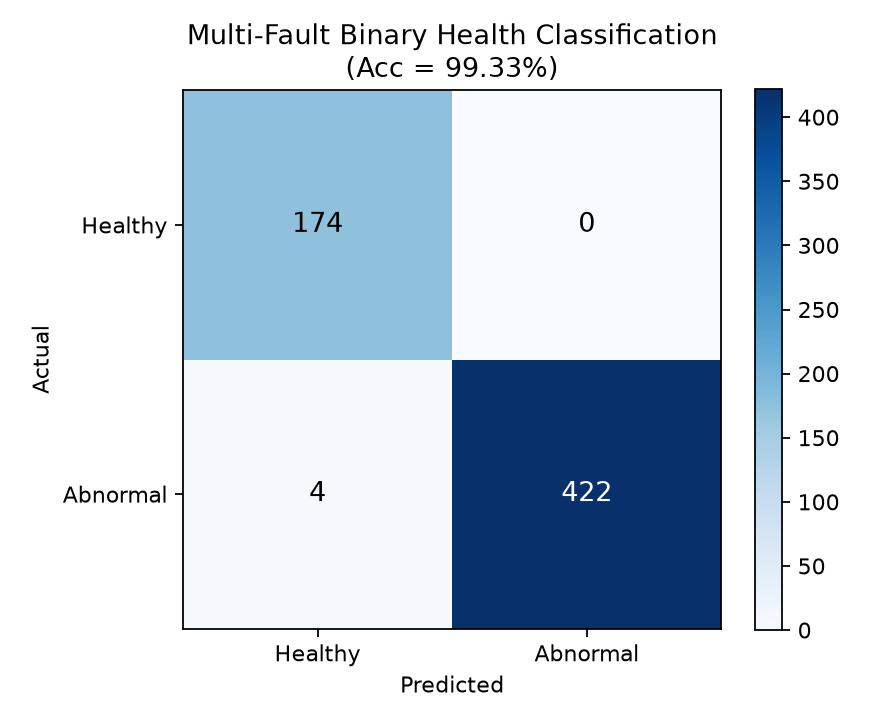
\includegraphics[width=\textwidth]{confusion_matrix_multifault_binary.png}
        \caption{Binary health confusion matrix.}
        \label{fig:cm_multi_bin}
    \end{subfigure}
    \hfill
    \begin{subfigure}[b]{0.56\textwidth}
        \centering
        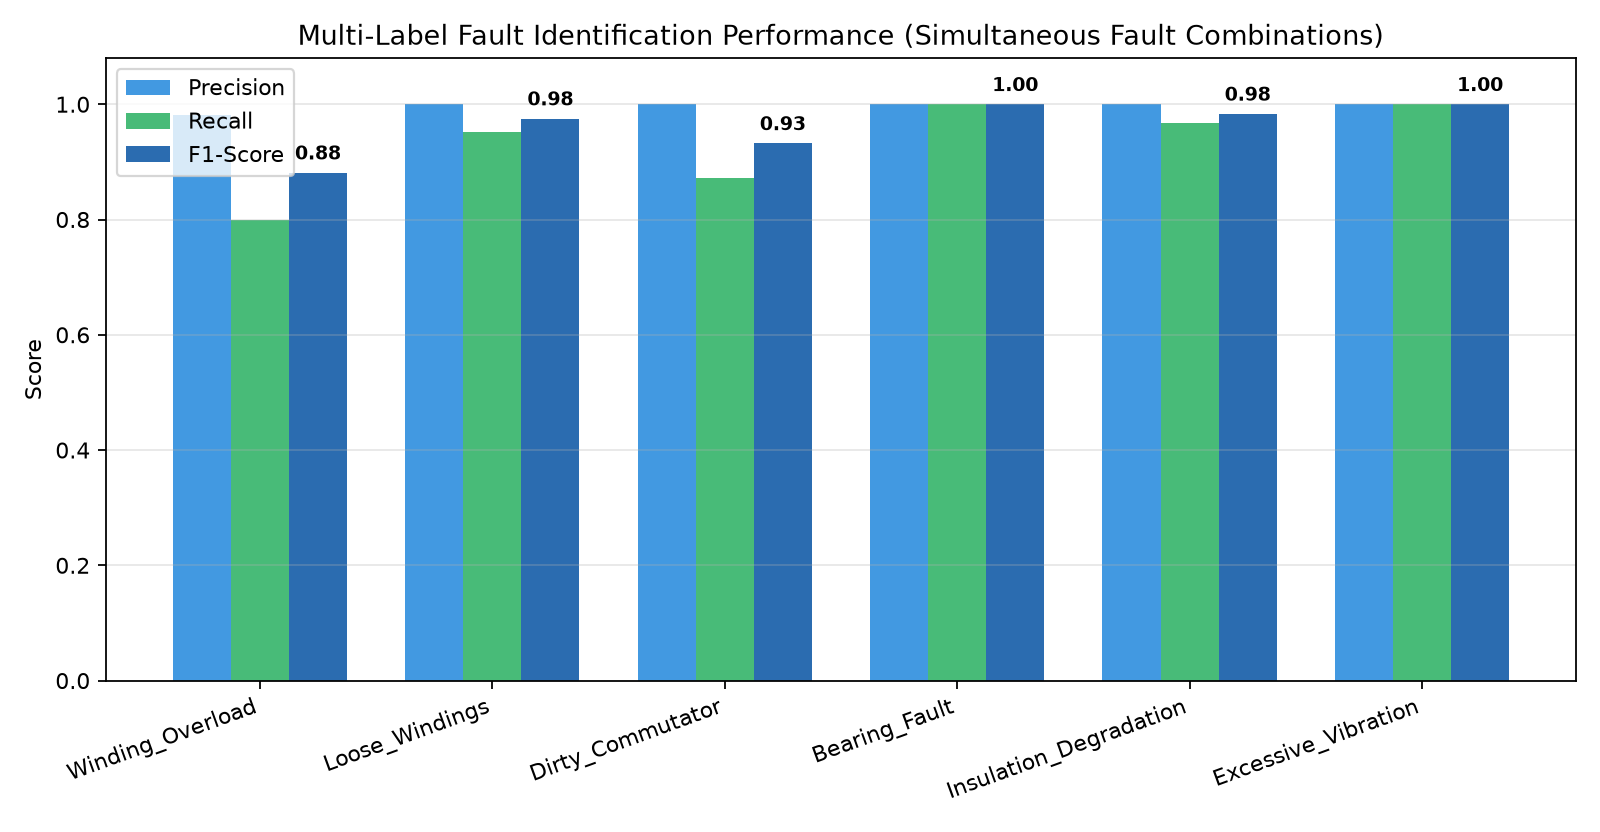
\includegraphics[width=\textwidth]{multilabel_f1_per_fault.png}
        \caption{Multi-label Precision, Recall, and F1 per fault.}
        \label{fig:ml_bars}
    \end{subfigure}
    \caption{Multi-fault binary detection and per-fault multi-label identification results.}
\end{figure}

\paragraph{Physical Interpretation of Errors and Improvement Over Prior Baseline}
As shown in Table~\ref{tab:multilabel_results} and Table~\ref{tab:exact_by_k}, exact-match accuracy steps down realistically from 100\% (Healthy) to 76.92\% (3 concurrent faults). Mechanical/spectral faults (\emph{Bearing Fault}, \emph{Excessive Vibration}, \emph{Loose Windings}) remain highly separable (F1 $\ge 0.975$) because they occupy distinct frequency bands. Conversely, mild \emph{Winding Overload} (Recall 80.0\%) and \emph{Dirty Commutator} (Recall 87.3\%) experience partial masking when co-occurring with bearing drag or insulation degradation, since all three elevate armature current and temperature rise. Overall, compared to our prior 100\,Hz time-domain baseline, binary accuracy improved from \textbf{85.83\% to 99.33\%}, multi-label macro F1 improved from \textbf{0.7694 to 0.9620}, and bearing/friction F1 improved from \textbf{0.4946 to 1.0000}.

%======================================================================
\section{Laboratory Deployment, Safety, and Hardware Plan}
%======================================================================

\subsection{Safe and Reversible Fault Induction in a College Lab}

Destructive testing cannot be performed on a college Electrical Machines Lab DC motor. Fault verification is therefore structured into three safety tiers:
\begin{itemize}[leftmargin=*, itemsep=3pt]
    \item \textbf{Tier A (Directly Inducible \& 100\% Reversible):}
    \begin{itemize}[noitemsep]
        \item \emph{Winding Overload:} Load the motor to 110--130\% rated current for 2--5 minutes using the lab's brake drum or coupled DC generator lamp/rheostat bank, stopping below $55\text{--}60^\circ\text{C}$ casing temperature.
        \item \emph{Excessive Vibration:} Clamp a small known mass onto the coupling/brake drum behind a guard (unbalance), slightly loosen one base bolt by $1/2$ turn with a locknut (soft-foot), or insert a $0.5\text{--}1.0\,\text{mm}$ shim at the flexible coupling (misalignment, with technician approval).
    \end{itemize}
    \item \textbf{Tier B (Safe External Proxies / Spare-Rig Testing):}
    \begin{itemize}[noitemsep]
        \item \emph{Dirty Commutator:} Insert a high-wattage low-ohm rheostat ($0.2\text{--}1.0\,\Omega$) in series with the armature to emulate elevated brush contact resistance (never contaminate a healthy lab commutator).
        \item \emph{Bearing Fault:} Test physically notched or grease-depleted 6204/6205 bearings only on a low-cost spare benchtop motor or removable end-bell housing; on the main lab motor, light brake-drum drag can serve only as a friction-only proxy.
    \end{itemize}
    \item \textbf{Tier C (Never Induce Directly):}
    \begin{itemize}[noitemsep]
        \item \emph{Insulation Degradation:} Never short or burn lab windings. Use the lab's field rheostat to emulate flux weakening ($K_e\Phi$ reduction) and use a 500\,V DC Megger offline to verify baseline insulation resistance.
        \item \emph{Loose Windings:} Validate via simulation, or temporarily couple a small external 100/200\,Hz vibration exciter onto the casing to verify the accelerometer FFT pipeline.
    \end{itemize}
\end{itemize}

\subsection{Operating Without Real Physical Fault Data (Two-Stage Hybrid Strategy)}

Because destructive fault data will not be available from the college lab motor during initial hardware integration, we propose a \textbf{two-stage hybrid monitoring architecture} widely used in industrial predictive maintenance:
\begin{enumerate}[leftmargin=*, itemsep=3pt]
    \item \textbf{Stage 1 — Healthy-Only Anomaly Detection (Zero Fault Data Required):} Record 15--30 minutes of real \emph{Healthy} operation across normal speeds and loads (no-load to 100\% rated load). Train an unsupervised anomaly detector (Isolation Forest or Mahalanobis distance) exclusively on this real healthy baseline so it learns the exact noise floor, rectifier ripple, and structural resonances of the physical lab motor. Any real deviation immediately triggers an \emph{Abnormal} alert.
    \item \textbf{Stage 2 — Calibrated Digital Twin \& Residual Diagnosis:} Calibrate the simulator's nominal parameters ($R_a, L_a, K, B$, baseline vibration, thermal curve) to match the measured healthy lab motor, and compute \emph{residual features} ($\Delta I_a$, normalized FFT ratios relative to healthy baseline). When Stage 1 flags an anomaly, the Extra Trees model trained on the calibrated digital twin acts as a diagnostic advisor—validated live in front of faculty using the safe reversible Tier A perturbations (overload and unbalance/looseness).
\end{enumerate}

\subsection{Proposed Bill of Materials (BOM) for the 220 V Lab Motor}

Unlike low-voltage hobbyist IoT prototypes~\cite{chougule2026}, a 220\,V DC lab motor strictly requires \textbf{galvanically isolated transducers}, a \textbf{high-bandwidth 3-axis MEMS accelerometer} (for 500\,Hz FFT analysis), and a \textbf{battery-powered wireless DAQ} so the laptop is never electrically tied to the motor circuit.

\begin{table}[H]
\centering
\small
\setlength{\tabcolsep}{4pt}
\caption{Proposed Bill of Materials (BOM) for the wireless 220\,V DC motor monitoring DAQ.}
\label{tab:bom}
\renewcommand{\arraystretch}{1.15}
\begin{tabular}{@{}cp{0.31\textwidth}cp{0.36\textwidth}c@{}}
\toprule
\textbf{\#} & \textbf{Component / Spec} & \textbf{Qty} & \textbf{Purpose} & \textbf{Est. INR} \\
\midrule
1 & Raspberry Pi Pico W (or ESP32) & 1 & 500\,Hz sensor DAQ \& Wi-Fi streaming & 650 \\
2 & Isolated DC Voltage Transducer (LEM LV 25-P / 0--300\,V DC to 0--3.3\,V, $\ge 2$\,kV) & 1--2 & Safe isolated $V_a$ (and optional $V_f$) measurement (do \emph{not} use AC-only ZMPT101B) & 2,000--4,500 \\
3 & Isolated DC Current Transducer (ACS758LCB-050B 50\,A / LEM LA 55-P) & 1--2 & Isolated $I_a$ measurement with bandwidth for commutation ripple & 800--2,500 \\
4 & External SPI ADC (MCP3008, 10-bit) & 1 & Fast multi-channel sampling of $V_a, I_a$ at $\ge 500$\,Hz & 350 \\
5 & 3-Axis MEMS Accelerometer (ADXL345, SPI up to 3.2\,kHz) & 1 & Bearing kurtosis \& $1\times$/$2\times$/100\,Hz vibration FFT (rigidly mounted on drive-end housing) & 300 \\
6 & MLX90614 Non-Contact IR Temp Sensor & 1 & Motor casing / commutator surface temperature & 650 \\
7 & DS18B20 / MAX6675 K-Type Thermocouple & 1 & Direct bearing end-bell temperature & 250 \\
8 & TCRT5000 IR Tachometer (or A3144 Hall) & 1 & Non-contact shaft RPM for harmonic tracking & 150 \\
9 & 5\,V USB Power Bank (10,000\,mAh) & 1 & Galvanically floats the DAQ from mains earth & 900 \\
10 & ABS IP65 Enclosure, 600\,V CAT III Shrouded Leads, 1\,A Inline Fuse, Mounts & 1 set & Electrical protection \& repeatable sensor mounting & 1,200 \\
\midrule
\multicolumn{4}{r}{\textbf{Estimated Core DAQ Total}} & \textbf{7,250--11,450} \\
\midrule
11 & \emph{(Optional)} 24--48\,V Spare DC Motor + 2$\times$ 6204 Bearings + 1\,$\Omega$/100\,W Resistor & 1 set & Dedicated benchtop rig for physical bearing-notch and brush-wear tests & 2,500 \\
\bottomrule
\end{tabular}
\end{table}

\subsection{Limitations and Next Steps}
All accuracy metrics in this report are obtained strictly from physics-based synthetic data and represent a \textbf{simulated upper bound} confirming feature separability. Physical phenomena such as magnetic saturation, structural transfer-function resonances, sensor drift, and real brush-arcing EMI will reduce raw zero-shot accuracy until the hardware DAQ is deployed, calibrated on healthy lab recordings, and validated experimentally.

%======================================================================
\begin{thebibliography}{9}
\bibitem{yousefnejad2025}
S.~Yousefnejad, F.~Bagheri, R.~Alshawi, M.~T.~Hoque, and E.~Amiri,
``Deep Learning Based Fault Detection Method in DC Motor Start,''
\emph{IEEE Transactions on Energy Conversion}, vol.~40, no.~2, pp.~1678--1681, Jun.~2025.

\bibitem{chougule2026}
R.~Chougule, S.~Bhosale, T.~Badave, S.~Jadhav, and M.~S.~Chavan,
``DC Motor Fault Detection Using IoT,''
\emph{International Journal of Research Publication and Reviews (IJRPR)}, vol.~7, no.~5, pp.~12453--12456, May~2026.
\end{thebibliography}

\end{document}
